\section{Introduction}

In its first 10 years of observations, the Rubin Observatory will perform the Legacy Survey of Space and Time (LSST), as described
in Ref.~\citenum{2019ApJ...873..111I}. In the construction phase of the observatory, the Data Management subsystem,
described in Ref.~\citenum{2015arXiv151207914J}, is in charge of developing and preparing the
software, services, and systems that will automatically reduce the raw data to produce science-ready data products.
Project requirements on DM products are documented in change-controlled specifications. DM Verification and Validation(V\&V)
activities are planned to guarantee that survey software and infrastructure both fulfill the system requirements
and enable the science that motivates the project.

We present here the tooling and procedure used at the Rubin Observatory for the documentation of verification and validation activities.
These are an evolution of the approach to the same use case, adopted 
for the Gaia Data Processing and Analysis Consortium (DPAC) project, described in Ref.~\citenum{10.1117/12.926797}.
Test activities are managed in Jira: test cases are created and updated, and test results are reported. 
This ensures that all elements to be documented (e.g., Requirements or Verification Elements) 
are available in one tool and that their history is maintained.
The Systems Engineering model is synced with the Jira test framework, providing a direct link between
tests and system requirements. Test documents can therefore be generated automatically, avoiding typical problems
such as lack of traceability, typographical errors, duplication of content, and misalignment between documents. The
centralized collection of information permits a high level of automation, where the extraction of test documents is
achieved by a continuous integration process. This systematic approach substantially reduces the time required to
produce verification and validation documentation, and its integration with the project's Systems Engineering model,
detailed in Ref.~\citenum{10.1117/12.2310125}, ensures full traceability to system requirements. 
This approach becomes even more necessary if we look at the number of requirements that need to be verified and documented, 
approximately 700 only for Data Management.

To complete the picture, a description of each document involved in the process is given. These documents are: 
the \textit{Test Specification} documents to baseline the test cases, 
the \textit{Verification Elements Baseline} documents to baseline the Verification Elements, 
the \textit{Test Plan and Report} documents providing test campaign planning and reporting information,
and the \textit{Verification Control Document} that, using the same approach and information already available in Jira, 
becomes a useful document to measure internal progression and completion to the requirements coverage 
and an important document to include in review's data pack. 

In summary, Section \ref{sec:vandvproblem} introduce the Rubin Observatory Verification and Validation activities.
In Section \ref{sec:approach} we provide a description of the adopted approach, tools, documents, and procedures. 
Section \ref{sec:vcd} introduces the Verification Control Document. 
Finally in Section \ref{sec:conclusions} a few considerations on the implemented approach are provided.


\section{The Verification And Validation Context}
\label{sec:vandvproblem}

The purpose of the verification and validation activities is to ensure that all requirements have been properly implemented and verified,
or deviation and non-conformances have been documented and approved.
This includes identifying the requirements, the affected components, and the verification procedures.

Figure \ref{fig:topdoctree} shows the flow down of high level requirements documents.
The Data Management requirements are baselined in the Data Management System Requirements\cite{LSE-61}, also known as the DMSR.
The DM requirements are flowed down from the System Science Requirements Document (SRD)\cite{LPM-17}. Interface requirements between DM and other Rubin Observatory subsystems also impact Data Management provided components and, therefore, need to be considered during Verification and Validation.

\begin{figure}
\begin{center}
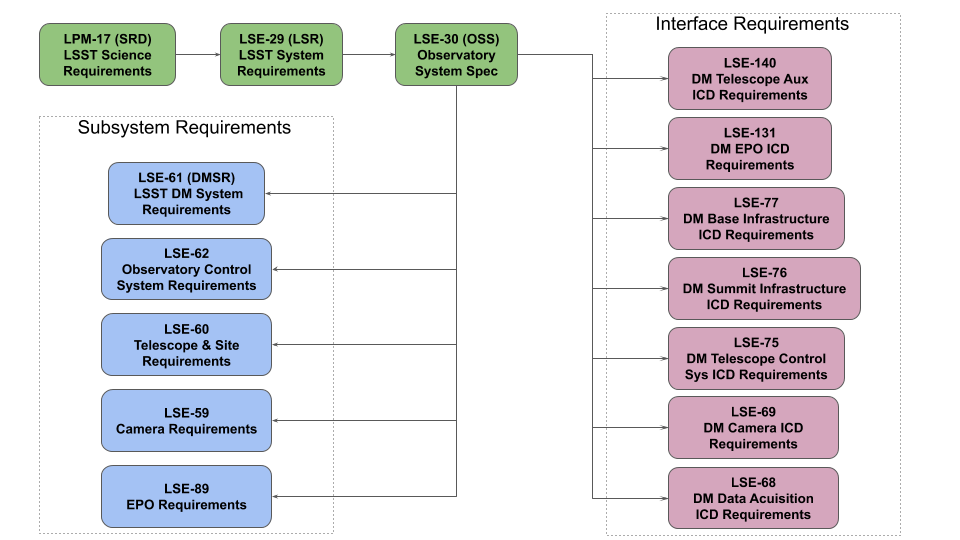
\includegraphics[width=\textwidth]{imgs/TopLevelDocTree.png}
 \caption{The Rubin Observatory top level document tree. In green the top-level requirements documents,
in blue the LSST subsystem's requirements documents and in red the DM related interface requirements documents }
 \label{fig:topdoctree}
\end{center}
\end{figure}

DM is responsible for both, fully verifying the DMSR requirements and contributing to the verification and validation of those interface requirements that have an impact on the DM subsystem.
To achieve this, we create one or more Verification Elements for all requirements.
These Verification Elements are assigned to the validation scientist,
who will ensure they are properly described and are sufficient to fully verify the corresponding requirements.
The validation scientist will also ensure that for each Verification Element there is at least one associated test case.
In the case that the provided Verification Elements are not sufficient, the validation scientist will request additional Verification Elements to be associated with the requirement.
In the opposite case, if a provided Verification Element is not needed, it will be removed.
Figure \ref{fig:vandvschema} shows the relationships between requirements, Verification Elements, test cases and results.

The verification and validation activities are organized into test campaigns, each of which is associated with one milestones\footnote{A 
milestone is a set of functionality or activities, that are expected to be implemented or completed at a specific point in time. 
In the context of V\&V, milestones are defined as Jira issues. Their definition and management is not in the scope of this paper.},
The results of the test executions are collected in Jira and coverage information is propagated back to the Verification Elements and requirements in the system engineering model.
Test documents, including test reports, are generated automatically from Jira.

\begin{figure}
\begin{center}
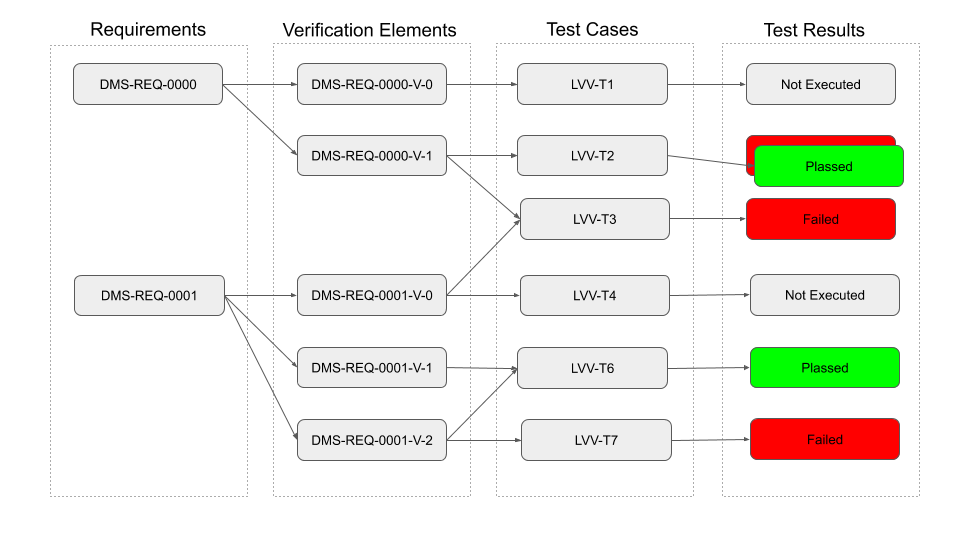
\includegraphics[width=\textwidth]{imgs/VandVSchema.png}
 \caption{Schematic approach to the Verification and Validation.}
 \label{fig:vandvschema}
\end{center}
\end{figure}

This approach ensures that all elements required for the tests are linked and available in Jira, 
providing traceability and making it possible to extract the necessary information into test documents without manual intervention.


\section{TheVerification and Validation Approach}
\label{sec:approach}

The verification and validation approach as illustrated in  Ref.~\citenum{10.1117/12.2310125}  has been implemented.
Required tools like \textit{Syndeia} and \textit{Docsteady} have been put in place.
Others tools used in the process described in \ref{sec:proc}, are also generally used in other project activities.


\subsection{The Tools Used}

\begin{figure}
\begin{center}
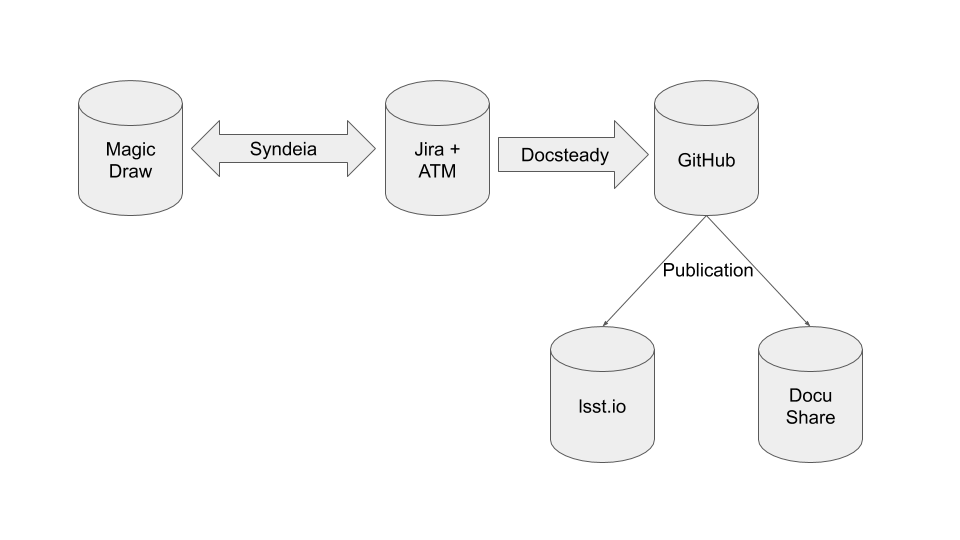
\includegraphics[width=\textwidth]{imgs/VandVtools.png}
 \caption{Schematic overview of the tools involved in the V\&V process.}
 \label{fig:vandvtools}
\end{center}
\end{figure}

We provide in this subsection a short description for the tools involved in the Verification and Validation activity.
Figure \ref{fig:vandvtools} provides a schematic overview of the tools, while
Figure \ref{fig:overview}  shows a few screenshots of the tools as implemented at Rubin Observatory.
We can see how Verification and Validation information flows from Jira, where it is created and maintained,
to the final document ready to be uploaded to DocuShare, the official Rubin Observatory documentation repository. 


\paragraph{MagicDraw}
is the Rubin Observatory modeling tool. It maintains the project models and requirements,
using a Model Based Systems Engineering (MBSE) approach.
The Verification Elements are created in MagicDraw using the requirements as a starting point,
and are synchronized to and from \textbf{Jira} using \textbf{Syndeia}.
This ensures that the proper traceability between requirements and Verification Elements is in place,
and that changes in one part of the system can be propagated through other components.

\paragraph{Jira}
is the Rubin Observatory issue tracking system.
The \textit{Test Manager for Jira} plugin (TM4J), previously known as \textit{Adaptavist Test Manager} (ATM),
provides additional functionality to Jira to manage test activities.
Jira hosts all test information, providing an easy-to-use graphical interface to the user.

\paragraph{Syndeia}
is a third party tool that integrates \textbf{MagicDraw} and \textbf{Jira}. 
First the Verification Elements are created in MagicDraw and then the data is synced to Jira
via a mapping between the fields in MagicDraw and the fields in Jira, utilizing the REST API.
After the test activity is completed, the information will be synced back to MagicDraw.

\paragraph{Docsteady}
is the tool that generates the test documents, extracting the information from Jira using the REST API.
It can be executed manually -- from the command line -- or automatically -- in a continuous integration (CI) tool --
and generates the documents in \LaTeX~format.
Using a CI system such as Jenkins, verification and validation documents can be generated continuously, or on a regular basis.
The extracted \LaTeX~ code is managed in Git repositories.
Docsteady is developed by the DM subsystem and the source code is available at \url{https://github.com/lsst-dm/docsteady}.

\paragraph{GitHub}
is the platform used for software version management.
Verification and Validation documents are written in \LaTeX~and maintained in Git repositories.
Whenever an author pushes changes to GitHub, a cloud-based continuous integration service 
(typically Travis CI) renders a pdf of the document and uploads it to \textbf{LSST the Docs}.

\paragraph{LSST the Docs}
is the Rubin Observatory documentation hosting platform, see The LSST the Docs Platform for Continuous Documentation Delivery\cite{SQR-006}.
LSST the Docs hosts not only the accepted version of a document on its own subdomain of \texttt{lsst.io}, but also draft and
historical versions corresponding to Git branches and tags.
By publishing draft updates of documents in near-real-time, teams can collaborate and comment on documents without having to
compile them locally.
LSST the Docs hosts any type of static web content.
To specifically publish pdf documents, we run a tool within the continuous integration service called \textit{Lander}
(available at \url{https://github.com/lsst-sqre/lander})
that generates an HTML landing page for the pdf based on metadata extracted from the document's source.

\paragraph{DocuShare}
is the official Rubin Observatory documentation repository during construction.

\begin{figure}
\begin{center}
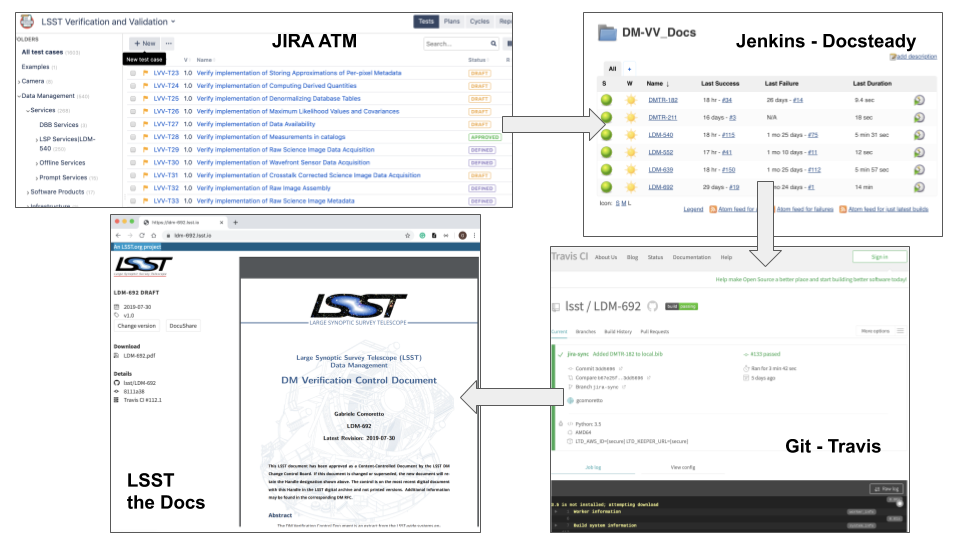
\includegraphics[width=\textwidth]{imgs/screenshots.png}
 \caption{Tools workflow overview: bringing information from Jira \textit{TM4J} to the published document available on the web. The information in Jira is synched with the system engineering model in MagicDraw.}
 \label{fig:overview}
\end{center}
\end{figure}


\subsection{Process Overview}\label{sec:proc}

All Verification and Validation activities derive from the requirements.
We assume in this document, that the requirements have been properly formalized, documented, and approved, 
see Ref.~\citenum{10.1117/12.2310125}.
As described early in this paper, a defined number of Verification Elements are created for each requirement.
When first created, the Verification Elements have no description;
the only information they contain is the details of the requirements from which they were generated.
They are synced to Jira using Syndeia, after which the validation scientist ensures that they are properly addressed.
Figure  \ref{fig:vandvproc} gives a graphical overview of the process.

\begin{figure}
\begin{center}
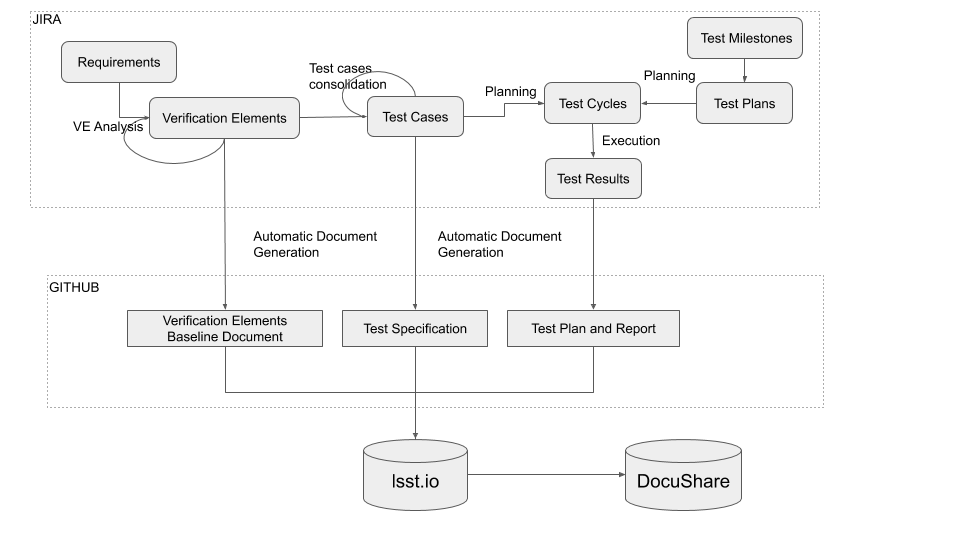
\includegraphics[width=\textwidth]{imgs/VandVprocedure.png}
 \caption{Schematic overview of the V\&V procedure.}
 \label{fig:vandvproc}
\end{center}
\end{figure}

The following subsections describe the main steps of the verification and validation activities that take place in Jira.


\subsubsection{Verification Elements Analysis}

The first activity, required before starting with any test campaign, is to ensure that each Verification Element 
is complete and contains all the relevant information.
This is done by the validation scientist, or designee.

In this phase, the Verification Elements shall be completed with the following information:
\begin{itemize}
\item the description, which clarifies the scope of the Verification Element, that is, which part or parts of the requirement will be verified.
\item one or more draft test cases, each of which are defined with a one-sentence objective and an owner. 
In this way each test case is automatically traced to a Verification Element and therefore to a requirement.
\end{itemize}
Verification Elements are baselined in a \textit{Verification Baseline Document}.


\subsubsection{Test Case Consolidation}

The owner of each test case is responsible for completing it and providing in Jira all relevant information, like for example 
the objective of test, the pre and post-conditions, and a the test procedure with the steps to execute during the test campaign.
Additional test cases can be created as needed. All test cases are related to a Verification Element in order to guarantee the traceability.
In general, test cases can be associated with multiple Verification Elements, and therefore with more than one requirement.

Test cases should be general, specifying only the software component or the dataset type required.
The exact software and/or dataset versions and the configuration to be used during the test
is provided in the test campaign planning phase.
Test Cases are baselined in \textit{Test Specifications}.

\subsubsection{Planning and Execution}

As described in Section \ref{sec:vandvproblem} all test activities are organized into test campaigns.
For each test campaign, two \textit{TM4J} objects are created:

\begin{itemize}
\item \textbf{TM4J Test Plan} that provides the context of the test activity, and typically corresponds to a project milestone.
\item \textbf{TM4J Test Cycle}(s) that provides the scope of a subset of tests to be executed. For each test campaign we may have multiple test cycles,
with different configurations, datasets, or extra conditions we may want to test. Each Test Cycle is traced
to the TM4J Test Plan, and provides the list of test cases that need to be executed within that scope.
\end{itemize}

For each test campaign we identify two phases:

\paragraph{Planning}
This is the preparation phase of the test campaign. All relevant information, e.g. software version, datasets to use, 
hardware or configuration, is  collected in the two \textit{TM4J} objects defining the test campaign:  the Jira Test Plan and the Jira Test Cycle(s).
At the successful completion of this phase the test is ready to start.

Rubin Observatory does not instigate a formal Test Readiness Review for each test campaign,
however the tooling and procedures in place permit the person who is responsible for the test activity, and relevant stakeholders, to assess and review the collected information.
This is done by extracting the information into a document, the \textit{Test Plan and Report}, in GitHub, generating the pdf and making it available
in the corresponding LSST the Docs landing page. The Product Owner\footnote{The Product Owner is in charge of a product and owns the outcome, ensuring it is in line with the requirements.}, contributors and stakeholders can easily access the produced pdf,
check the content of the Test Plan, and comment, ask for clarification, or request changes using the GitHub
Pull Request (PR) mechanism or the corresponding Jira issue. 
When agreement has been reached, the TM4J Test Plan status is changed to \textbf{Approved} to indicate the test activity is ready to start.

The approved \textit{Test Plan and Report} document resulting at the end of this first phase, has to be uploaded to DocuShare 
as a reference for the next phase. The document at this stage provides the agreed test procedures and all the necessary 
information required to execute the tests.

\paragraph{Execution}
In this phase, the testers, identified in the previous phase, execute the test procedures and
document the result of each step in Jira.
The \textit{TM4J} plugin provides a test player view, where for each step in each test case, it is possible to say if it has been executed successfully or not,
specifying the result of the step, and associating any Jira issues that have been found during the test execution.

The test result information is extracted and added to the \textit{Test Plan and Report} document.
Once the test execution is complete, an overall assessment must be provided in the \textit{TM4J} Test Plan.

As in the previous phase, the document is generated automatically from Jira and provides an easy way to access the test campaign information.
Product owner, contributors and stakeholders can review the outcome of the test campaign 
using the same GitHub PR mechanism reported above, commenting, asking for more information, or changes if required.
Finally, the Product Owner is in charge of approving the test campaign result, when they considers that the collected information is complete.

The \textit{TM4J} Test Plan status will then be changed to \textbf{Done}.
At the end of the test campaign, the  final \textit{Test Plan and Report} is issued and uploaded to DocuShare.
We can assume that, in special cases, the document can be used to document further executions in the context of the same test campaign.
For example, in the case the test campaign verifies a specific software release, a future patch on that software release can be tested
with the addition of a specific Test Cycle to the \textit{TM4J} Test Plan.
However, future test campaigns will use completely new test plan and report document


\subsection{Test Documents}

The documents identified in the above steps are generated using Docsteady.
The generation can be done manually or automatically.
Automation is particularly useful if we want to see daily progress published on the LSST the Docs landing page.

The extraction tool ensures homogeneity of information at all levels in the Verification and Validation activities,
and allows the user to concentrate only on the relevant test activities, without the need to worry about any documentation aspects.

The test documents are:

\begin{itemize}
\item \textbf{Test Specification}:  baselines the test cases.
A new issue of the document is made each time there is a substantial change in the definition of test cases.
\item \textbf{Test Plan and Report}:  for a single test campaign this includes all planning and execution information.
It is issued at least twice. The first issue corresponds to the consolidation of the planning activity,
the second to the finalized test campaign containing the results of the same.
\item \textbf{Verification Baseline Document}: provides a snapshot of the Verification Elements.
The Verification Elements are  maintained as Jira issues, and  thus are easy to change.
Having a snapshot of the Verification Elements at a specific point in time  (in the form of a document) makes
for a stable baseline and is good for tracking changes.
Approved versions are uploaded in DocuShare and used as a reference in other test documents.
\end{itemize}

Test Specifications and Verification Baseline documents are created for specific components, where components are the main products in a subsystem.


\section{The Verification Control Document}
\label{sec:vcd}

The Verification Control Document (VCD) provides an overview layer that summarize all V\&V activities.
Therefore it is an important management tool for assessing the level of verification and validation that has been achieved to date.
It is also useful to include it in review documents packs, to show which requirements have been verified.

Given that all information pertaining to V\&V activities is stored in Jira, the VCD can easily be extracted on-demand using the document generation tool Docsteady.
As for all other test documents, the VCD is a \LaTeX~document, managed in a GitHub repository, built with Travis CI and published through LSST the Docs.

Given that both the number of requirements and Verification Elements for Rubin Observatory is very high --
approximately 700 requirements and 1000 Verification Elements in DM alone -- a separate VCD is generated for each subsystem.

There are two main sections to the VCD:

\begin{itemize}
\item \textbf{Summary Information} where a status overview is given.
This includes the number of requirements and Verification Elements covered by passed (successfully executed) test cases.
Figure \ref{fig:vcdsum} shows an example extracted from the DM VCD.
\item \textbf{Detailed Information} where for each requirement, the Verification Elements, test cases
and the status of the test cases are shown. Links to the test documents are provided, but not descriptive information.
Figure \ref{fig:vcddetail} shows a detail example extracted from the DM VCD.
\end{itemize}

\begin{figure}
\begin{center}
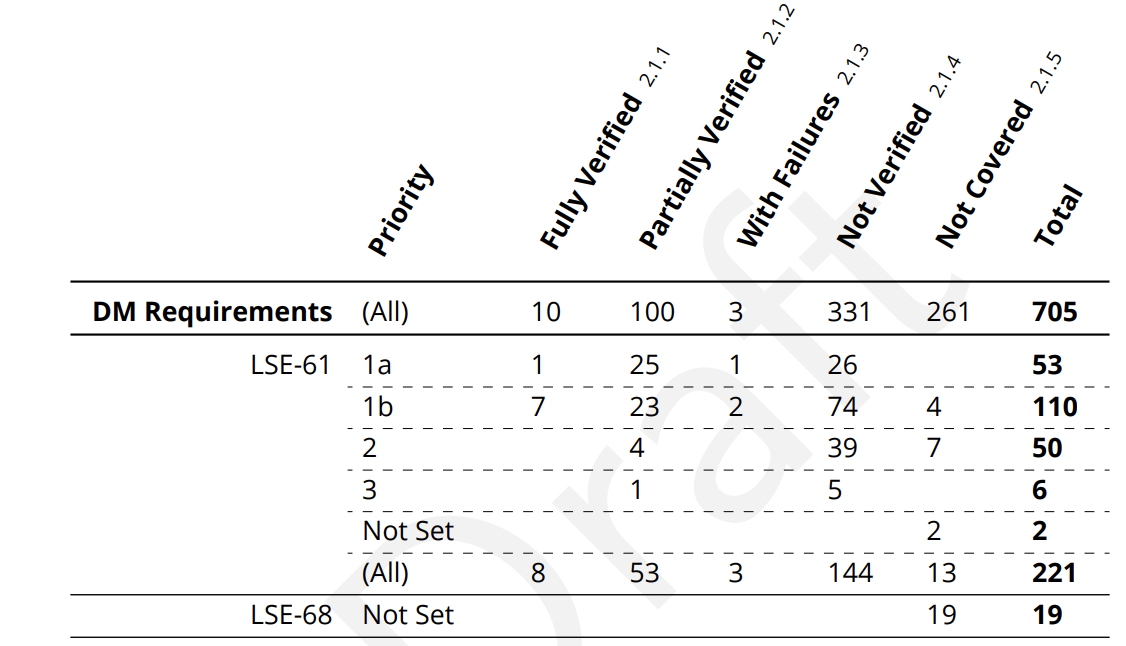
\includegraphics[width=\textwidth]{imgs/VCDsumm.png}
 \caption{Example summary extracted from the DM VCD. 
 Here we see summary for the DMSR \cite{LSE-61} and for the LSE-68 interface requirements specification\cite{LSE-68}.}
 \label{fig:vcdsum}
\end{center}
\end{figure}

\begin{figure}
\begin{center}
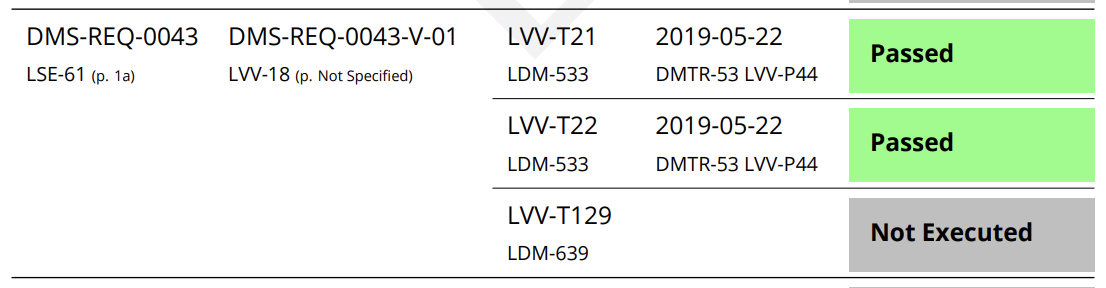
\includegraphics[width=\textwidth]{imgs/VCDdetail.png}
 \caption{Example of a detailed information for a requirement extracted from the DM VCD 
 showing a Verification Element and three test cases, of which two have been executed and passed.}
 \label{fig:vcddetail}
\end{center}
\end{figure}


\section{Conclusions and Outlook}
\label{sec:conclusions}

In the context of a large project like Rubin Observatory construction, with a large number of requirements
and subsystems/components, the presented approach shows how integrating custom tools like Docsteady
and Syndeia into the existing infrastructure significantly reduces the effort
required to produce verification and validation documentation.
This permits the team to concentrate on the relevant test activities, maximizing the scientific outcome.

At the same time, automation and continuous integration of the document generation makes test information
much more accessible to the users and stakeholders.
The tooling also ensures that aspects such as traceability between tests and requirements, homogeneity of the information
or reusability of test cases are easy to implement and provide added value to the process.

Finally, the VCD provides a global overview of all DM requirements, ensuring all DM direct and interfacing requirements are covered.

This approach is not only used by DM, but also by other Rubin Observatory subsystems that are facing the same challenge.
The VCD for the time being is only provided by DM, but the tooling and procedure are ready to serve all other Rubin Observatory subsystems.
Using the same tools permit everybody to use the same template and have the same documentation format across the project.


\acknowledgments
This material is based on work supported in part by the  {National Science Foundation} through Cooperative Agreement 1258333 managed by the  {Association of Universities for Research in Astronomy} ({AURA}), and the  {Department of Energy} under  {Contract} No.  {DE}-AC02-76SF00515 with the  {SLAC} National Accelerator Laboratory. Additional LSST funding comes from private donations, grants to universities, and in-kind support from LSSTC Institutional Members.

This research has made use of  NASA's Astrophysics Data System Bibliographic Services.
